\section{Messung}
\label{sec:messung}
Im Folgenden Abschnitt wird zunächst eine Energiekalibration der Apparatur durchgeführt. Anschließend werden mit der Aufnahme eines Cäsium-Strahlers verschiedene Detektoreigenschaften bestimmt.
Daraufhin wird die Aktivität einer ???-Quelle gemessen und schließlich einige Holzkohlebriketts auf ihre radioaktiven Bestandteile untersucht.

\subsection{Eichung und Effizienz des Ge-Detektors}
\label{subse:eichung}
Wie in Abschnitt \ref{sub:bestimmung_der_energie_und_der_aktivität_einer_gamma_quelle} erwähnt, liegen nach der Messung lediglich Informationen über einen Energiekanal vor, in dem ein Ereignis detektiert wurde.
Um das entsprechende Spektrum in der Dimension \si{keV} der Energie zu erhalten, wird den Kanälen $C$ mit einer lineare Kalibrationsfunktion $E(C)$ eine jeweilige Energie $E$ zugeordnet.
Mit der Steigung $m$ und einem Offset $b$ wird hierfür verwendet:%
%
\begin{align}
    \label{eqn:kalibration}
    E(C) = mC + b\,.
\end{align}

Zunächst wird das Spektrum eines $^{52}$Eu-Strahlers aufgenommen (Abb. \ref{fig:eu_uncalibrated}).
Um den Einfluss von Untergrundereignisse zu verringern, wird zudem eine Leermessung durchgeführt und die Einträge dieser Messung der einzelnen Kanäle von dem Spektrum des $^{52}$Eu-Strahlers abgezogen (Abb. \ref{fig:leermessung}).
\begin{figure}[htb]
    \centering
    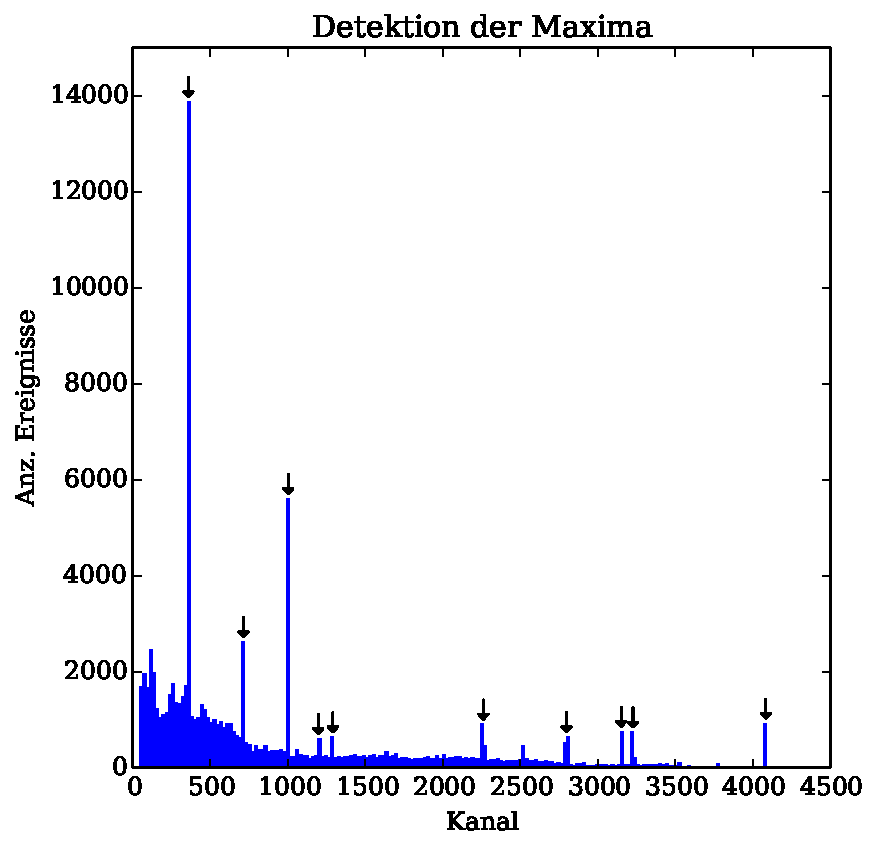
\includegraphics[width=0.8\textwidth]{img/02_maxima.pdf}
    \caption{

    }
    \label{fig:eu_uncalibrated}
\end{figure}
Die unterschiedliche Messdauer wird mit einem Faktor $t_\text{leer} / t_\text{Eu}$ der Messdauer $t_\text{Eu}$ des $^{52}$Eu-Strahlers und $t_\text{leer}$ der Leermessung berücksichtigt.
Dabei werden die in Tabelle \ref{tab:maxima} aufgeführten Maxima gewählt und den jeweiligen Kanäle mit Hilfe von \eqref{eqn:kalibration} eine Energie zugeordnet. Der Fit der Kalibratinosfunktion ist in Abbildung \ref{fig:calibration} dargestellt.
Es ergeben sich die Koeffizienten
%
\begin{align*}
     m = \SI{345.22+-0.04}{keV/C} \qquad b = \SI{-1.82+-0.09}{keV} \,.
\end{align*}

\begin{table}[htb]
    \centering
    \caption{
        Die für die Kalibration des Ge-Detektors verwendeten Maxima des $^{52}$Eu-Spektrums.
    }
    \label{tab:maxima}
    \begin{tabular}{rrr}
        \toprule
        Energie [\si{keV}] & Emissionswahrscheinlichkeit [\si{\percent}] & Zugeordneter Kanal \\
        \midrule
        \num{121.78} & \num{0.286} & \num{ 358} \\
        \num{244.7 } & \num{ 0.76} & \num{1003} \\
        \num{344.3 } & \num{0.265} & \num{ 714} \\
        \num{411.12} & \num{0.022} & \num{2262} \\
        \num{443.96} & \num{0.031} & \num{2798} \\
        \num{778.9 } & \num{0.129} & \num{4084} \\
        \num{964.08} & \num{0.146} & \num{3227} \\
        \num{1085.9} & \num{0.102} & \num{1291} \\
        \num{1112.1} & \num{0.136} & \num{3150} \\
        \num{1408.0} & \num{0.210} & \num{1196} \\
        \bottomrule
    \end{tabular}
\end{table}
